\chapter{Testy losowości}
\thispagestyle{chapterBeginStyle}

Rozdział ten poświęcony będzie testowaniu losowości wyników w celu ustalenia, czy liczby losowe otrzymane z naszego generatora spełniają warunek jednostajności oraz niezależności. Sprawdzimy, jak wypada on w stosunku do znanych rozwiązań. Opiszemy również teorię dotyczącą testowania losowości ciągów bitowych.

\section{Jak udowodnić losowość?}
Krótka odpowiedź brzmi na zadane w tytule niniejszego podrozdziału pytanie mówi, iż nie jest to możliwe. Aby móc powiedzieć z pewnością, jakimi parametrami cechuje się testowany generator, musielibyśmy poznać nieskończoność wygenerowanych przez niego wyników. Załóżmy, że wygenerował on do tej pory ciąg $N$ jedynek. Moglibyśmy rzucić zatem tezę, iż nie spełnia on założenia jednostajności. Wiemy że:
\begin{equation}
\begin{gathered}
    P(X = \mathbb{1}^N) = 2^{-N}\\
    \lim_{N \to \infty} P(X = \mathbb{1}^N) = \lim_{N \to \infty} 2^{-N} = 0
\end{gathered}
\end{equation}
Istnieje zatem szansa, że prawidłowy generator wyprodukuje taki ciąg. Żyjemy w skończonym świecie, a więc empiryczne sprawdzenie granicy dla $N$ dążącego do nieskończoności jest niemożliwe. Co za tym idzie, nie możemy matematycznie udowodnić, iż nie spełnia założeń.
\subsection{Redukcja oczekiwań}
Jesteśmy zmuszeni zatem  zredukować nasze oczekiwania odnośnie testowania generatorów, z matematycznego dowodu, do statystycznego prawdopodobieństwa. Nawiązując do poprzedniego przypadku wiemy, że uzyskanie wektora samych jedynek było zawsze możliwe, jednak szansa na to jest bardzo mała. Uzyskanie dowolnego $n$-elementowego wektora binarnego jest jednakowo prawdopodobne przy założeniu jednostajności i niezależności. Musimy zatem znaleźć jakąś funkcję mierzalną (w naszych zastosowaniach: w sensie Lebesqua), która nie będzie różnowartościowa i zmapuje wiele podobnych wektorów na tę samą wartość. Dobrym przykładem  będzie tutaj  np. stosunek zer do wszystkich cyfr. Jak nietrudno policzyć, dla generatora spełniającego założenie jednostajności, stosunek ten powinien wynosić $\frac{1}{2}$. Istnieją również tylko dwa najbardziej oddalone od tej wartości wektory: $\mathbb{1}^N$ i $\mathbb{0}^N$. Wiemy więc, że prawidłowy generator ma prawdopodobieństwo wylosowania tak skrajnie rzadko występującego przypadku równe $\frac{1}{2^{n-1}}$.
\section{Teoria testów statystycznych}
Test statystyczny jest to narzędzie pozwalające ocenić prawdopodobieństwo hipotezy statystycznej na podstawie skończonej próbki z pewnej populacji.
\subsection{Hipotezy statystyczne}
Każdy test zaczynamy od sformułowania hipotez:
\begin{description}
\item[hipoteza zerowa ($H_0$)] - podstawowa hipoteza mówiąca o tym, że próbka nie odbiega w żaden statystycznie istotny sposób od przyjętych założeń. W naszym przypadku oznacza to, że próbka została wygenerowana przez generator spełniający założenie jednostajności lub niezależności, albo oba.
\item[hipoteza alternatywna ($H_1$)] – zaprzeczenie hipotezy zerowej. W naszym przypadku hipoteza alternatywna będzie mówiła, że nasza próbka różni się w statystycznie istotny sposób od takich, które wygenerowałby generator spełniający założenie jednostajności lub niezależności, albo oba.
\end{description}

\subsection{Podstawowe definicje}
Wprowadzimy kilka podstawowych pojęć i symboli:
\begin{description}
\item[alfa ($\mathbf{\alpha}$)] - wartość określająca, jaka jest szansa, że generator spełniający hipotezę zerową nie przejdzie testu. Z reguły ustalona na poziomie 5\%.
\item[beta ($\mathbf{\beta}$)] – wartość określająca szansę, że generator spełniający hipotezę alternatywą uzyska pozytywny wynik testu.
\item[przedział ufności] – przedział w którym, zgodnie z rozkładem teoretycznym powinno znaleźć się $1-\alpha$ próbek. Tak jak na rysunku \ref{fig:confidence_interval} powinien on pokrywać najbardziej prawdopodobną część teoretycznego rozkładu. 
\end{description}
W przypadku testów statystycznych bardzo często dokonuje się uproszczenia modelu wykorzystując centralne twierdzenie graniczne zakładając, że populacja ma rozkład normalny. 
Ułatwia to znacząco wyznaczenie zakresów dla przedziałów ufności.
\begin{figure}[!htp]
    \centering
    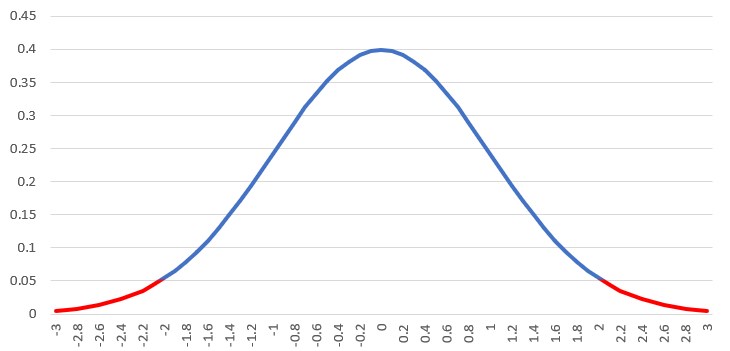
\includegraphics[width=10cm]{confidence_interval}
    \caption{Przedziały ufności(niebieski) dla testu statystycznego z cechą populacji mającą rozkład normalny z $\alpha=0.05$}
    \label{fig:confidence_interval}
\end{figure}
\subsection{Rodzaje błędów}
Przyswoiwszy znaczenie parametrów $\alpha$ i $\beta$ możemy powiedzieć kilka słów o rodzajach błędów, które możemy popełnić w naszym teście.

\begin{table}[!h]
\begin{center}
\begin{tabular}{cccc}
                                            &                          & \multicolumn{2}{c}{Rzeczywistość}                                          \\ \cline{3-4} 
                                            & \multicolumn{1}{c|}{}    & \multicolumn{1}{c|}{H_0}            & \multicolumn{1}{c|}{H_1}             \\ \cline{2-4} 
\multicolumn{1}{c|}{\multirow{2}{*}{Wynik}} & \multicolumn{1}{c|}{H_0} & \multicolumn{1}{c|}{Ok}             & \multicolumn{1}{c|}{Błąd II rodzaju} \\ \cline{2-4} 
\multicolumn{1}{c|}{}                       & \multicolumn{1}{c|}{H_1} & \multicolumn{1}{c|}{Błąd I rodzaju} & \multicolumn{1}{c|}{Ok}              \\ \cline{2-4} 
\end{tabular}
\end{center}
\caption{\label{tab:error_types} Przedstawienie rodzajów błędów w teście statystycznym}
\end{table}
Jak widzimy w tablicy \ref{tab:error_types}, wyróżniamy błąd pierwszego rodzaju (jeśli błędnie odrzucimy hipotezę zerową). Oraz błąd drugiego rodzaju (jeśli przymniemy hipotezę zerową pomimo iż byłą ona fałszywa).
\begin{table}[!h]
\begin{center}
\begin{tabular}{cccc}
                                            &                          & \multicolumn{2}{c}{Rzeczywistość}                                \\ \cline{3-4} 
                                            & \multicolumn{1}{c|}{}    & \multicolumn{1}{c|}{H_0}        & \multicolumn{1}{c|}{H_1}       \\ \cline{2-4} 
\multicolumn{1}{c|}{\multirow{2}{*}{Wynik}} & \multicolumn{1}{c|}{H_0} & \multicolumn{1}{c|}{1 - \alpha} & \multicolumn{1}{c|}{\beta}     \\ \cline{2-4} 
\multicolumn{1}{c|}{}                       & \multicolumn{1}{c|}{H_1} & \multicolumn{1}{c|}{\alpha}     & \multicolumn{1}{c|}{1 - \beta} \\ \cline{2-4} 
\end{tabular}
\end{center}
\caption{\label{tab:error_prob} Przedstawienie prawdopodobieństwa popełnienia błędu w teście statystycznym.}
\end{table}
Z tablicy \ref{tab:error_prob} możemy wyczytać iż $\alpha$ określa prawdopodobieństwo popełnienia błędu pierwszego rodzaju, a $\beta$ prawdopodobieństwo popełnia błędu drugiego rodzaju. O ile z łatwością możemy kontrolować $\alpha$ (wybierając inny przedział ufności, co możemy zobaczyć na rysunku \ref{fig:confidence_interval}), to kontrolowanie, a nawet wyliczenie $\beta$ jest w wielu przypadkach niemożliwe. 
Generatorów produkujących ciągi bitowe jest przynajmniej continuum. Dla każdej liczby rzeczywistej $p \in [0, 1]$ istnieje taki generator, że $(\forall i\in \mathbb{N})P(X_i=1) = p$. Załóżmy, iż mamy do czynienia z niezależnym generatorem o jakimś $p$ oraz, że $p$ zostało wybrane z rozkładem ciągłym. W takiej sytuacji, szansa wybrania $p = \frac{1}{2}$ wynosi dokładnie 0, a więc $\beta = 1$. Takie rozumowanie prowadzi jednak do poważenia zasadności testów statystycznych, przez co nie wyliczamy $\beta$, a jedynie skupiamy się na statystycznie istotnych różnicach.  
Możemy jednak stwierdzić, że dla coraz większej $\alpha$ zmniejsza się $\beta$. W skrajnym przypadku, gdzie $\alpha$ wynosi 1, $\beta$ będzie równa 0. Nie jest to jednak najbardziej użyteczny test, gdyż zawsze odrzuca on hipotezę zerową. Co więcej, o czy, nie należy zapominać, $\beta$ będzie zmniejszać się wraz z zwiększaniem się rozmiaru naszej próbki.
\subsection{Wartość $p$}
Kluczowym pojęciem w testach statystycznych jest wartość $p$ ($P_{\textrm{value}}$). Określa ona, w jakim miejscu teoretycznego rozkładu przy założeniu hipotezy zerowej znajduje się nasza próbka. Im większa wartość $p$, tym większe prawdopodobieństwo, iż została ona wzięta z populacji spełniającej hipotezę zerową, a w naszym przypadku: iż została wygenerowana przez jednostajny i niezależny generator. Obliczenie prawdopodobieństwa tego zdarzenia jak wiemy, jest jednak niezwykle trudne. Otrzymanie skrajnej wartości $p$ nie oznacza, że hipoteza zerowa jest fałszywa; oznacza jedynie, że jest mało prawdopodobna. Co więcej, przy założeniu prawdziwości hipotezy zerowej wartość oczekiwana wartości $p$ to $\frac{1}{2}$, gdyż dla $P_{\textrm{value}}(X) \sim \mathcal{U}(0, 1)$, gdzie $\mathcal{U}(0, 1)$ to rozkład jednostajny na odcinku $(0, 1)$. 
\section{Narzędzia testowania losowości}
Problem określania czy dany wektor bitów jest losowy czy nie, jest relatywnie starym problemem. Od czasów wykorzystywania liczb losowych w kryptografii pojawiło się wiele narzędzi do testowania oraz paczek testów.
\subsection{Przegląd paczek testów losowości}
\begin{description}
    \item[\textit{Ent}] - łatwa w użyciu paczka 5 testów losowości stworzona przez Johna Walkera w 1998 roku. Jest dostępna w dystrybucji Ubuntu. Zawiera dojść prymitywne testy, z których nie każdy posiada wyliczaną wartość $p$. Za pomocą tego narzędzia możemy przetestować wektor losowy dowolnej długości.
    \item[\textit{Diehard}] - pierwotnie wydany na płycie CD w 1995 roku przez George'a Marsaglię zestaw 12 testów na losowość stanowiący, jak na tamte czasy najlepszy tego typu pakiet. Jego użycie jest również proste. Nie zawiera on jednak satysfakcjonującego uzasadnienia matematycznego wykonywanych obliczeń oraz teoretycznego rozkładu, na podstawie którego wyliczane są wartości $p$. Narzędzie możemy znaleźć pod adressem \cite{Diehard}.
    \item[\textit{NIST test suite}] - zestaw 15 testów przygotowanych przez \textit{National Institute of Standards and Technology} w celu sprawdzenia generatorów liczb pseudolosowych do zastosowań kryptograficznych. Używane są jako standard dla kryptografii. Każdy z testów został opisany wa pracy \emph{A statistical test suite for random and pseudorandom number generatorsfor cryptographic applications} \cite{nist}. Zawarte w niej opisy testów nie zawierają sposobu wyliczenia teoretycznego rozkładu. Narzędzie to możemy znaleźć pod adresem \cite{NISTTests}.
    \item[\textit{TestU01}] - najnowsza wersja tej paczki testów pochodzi z 2009 roku, została stworzona przez Pierre L'Ecuyera. Jest ona również powszechnie używana, jednak została przygotowana do testowania generatorów liczb pseudolosowych i wymaga wbudowania swojego generatora w napisany języku w C framework testujący. Narzędzie możemy znaleźć pod adresem \cite{TestU01}.
    \item[\textit{Dieharder}] - narzędzie do testowania losowości stworzone przez Roberta G. Browna. Jego najnowsza wersją powstała w 2020 roku. Paczka zawiera testy z narzędzia \emph{dierhard}, jak również większość przygotowanych przez \emph{NIST} oraz autorskie testy. Jest narzędzie to jest dostępne w dystrybucji Ubuntu oraz pod adresem \cite{Dieharder}. Większość z nich wymaga dużej ilości danych powyżej 100MB. 
\end{description}
\subsection{Wybór generatorów do porównania wyników}
Nasze wyniki porównamy z trzema innymi znanymi generatorami różnej klasy. Przyjrzymy się jak wypada on na tle następujących rozwiązań:
\begin{description}
    \item[\textit{LCG} (\textit{Linear congruential generator})] - jedno z najstarszych i najbardziej znanych podejść do problemu generowania liczb losowych. Logika stojąca za tym generatorem jest łatwa do zrozumienia i sprowadza się do jednego wzoru:
    \begin{equation}
        \label{eq:lcg}
        X_{n+1} = (aX_n + b) \bmod m 
    \end{equation}
    Pomimo swojej prostoty daje on zadowalające wyniki, stąd też jest używany do dziś między innymi w bibliotece \emph{rand} języka C. Do testów użyjemy generatora o parametrach: $m=2^{32}$, $a=22695477$ oraz $b=1$.
    \item[\textit{Tarus}] - rozwiązanie bardzo zbliżone do poprzedniego stworzone przez Pierre L’Ecuyer'a. Posiada bardziej rozbudowany stan wewnętrzny składający się z trzech zmiennych: $s^1$, $s^2$ oraz $s^3$. Zasadę działania generatora opisuje wzór:
    \begin{equation}
        \label{eq:tarus}
        \begin{split}
            X_n &= (s^1_n \oplus s^2_n \oplus s^3_n)\\
            s^1_{n+1} &= ((s^1_n \mathbin{\&} 4294967294) \ll 12) \oplus (((s^1_n \ll 13) \oplus s^1_n) \gg 19)\\
            s^2_{n+1} &= ((s^2_n \mathbin{\&} 4294967288) \ll 4) \oplus (((s^2_n \ll 2) \oplus s^2_n) \gg 25)\\
            s^3_{n+1} &= ((s^3_n \mathbin{\&} 4294967280) \ll 17) \oplus (((s^3_n \ll 3) \oplus s^3_n) \gg 11)
        \end{split}
    \end{equation}
    gdzie $\mathbin{\&}$ oznacza operator iloczynu bitowego (\emph{and}), $\oplus$ oznacza bitową sumę rozłączną (\emph{xor}), a $\ll$ oraz $\gg$ oznaczają operację przesunięcia bitowego, odpowiednio w lewo i prawo.
    \item[\textit{CRNG} (\textit{Cryptographic random number generator})] - generator liczb losowych do zastosowań kryptograficznych. W tej pracy używamy rozwiązania z pakietu \emph{secrets} z języka Python. Wykorzystuje on zebraną przez system operacyjny entropię w celu wygenerowania liczb ''prawdziwie'' losowych.  
\end{description}
\section{Testy losowości}
Ze względu na niezwykle ubogie matematyczne uzasadnienie poprawności testów w znalezionych gotowych narzędziach testujących, jak również ich przystosowanie do testowania generatorów liczb pseudolosowych, wykorzystamy w tej pracy własne testy. Będą on mocno inspirowane pracą \emph{NITS} \cite{nist} wzbogacone o odpowiednie uzasadnienie matematyczne.
\subsection{Test częstotliwości}
\subsubsection{Cel testu}
Ten test skupia się na sprawdzeniu, czy wektor bitów $X$ ma rozkład jednostajny, a więc czy stosunek zer do jedynek dąży do równej proporcji. Jest to jeden z prostszych testów. Polega on na wyliczeniu wspominanej proporcji, a następnie obliczeniu szansy jej otrzymania przy założeniu jednostajności generatora. 
\subsubsection{Matematyczne podstawy testu}
Pierwszym krokiem będzie różnowartościowe zmapowanie wektora $X$ na zbiór $\{-1, 1\}$, tworząc zmienną losową $Y_i = 2X_i - 1$. Jest ona specjalnym przypadkiem rozkładu \ref{eq:dist}, z $p$ równym $\frac{1}{2}$. Korzystając z centralnego twierdzenia granicznego możemy użyć aproksymacji \ref{eq:norm_dist_avg} w postaci:
\begin{equation}
    \mathcal{N}\left(0, \frac{1}{\sqrt{n}}\right)
\end{equation}
Oznaczmy sumę po wszystkich wartościach $Y_i$ jako $S$:
\begin{equation}
    S =\sum_{i=1}^{n}(2X_i-1) = \sum_{i=1}^{n}Y_i
\end{equation}
Oznaczmy dodatkowo $\Phi$ jako dystrybuantę standardowego rozkładu normalnego:
\begin{equation}
    \Phi(x) = \int_{-\infty}^x\frac{1}{\sqrt{2\pi}}e^{-\frac{t^2}{2}} dt = \frac{1}{2}\left(1+ \textrm{erf}\left(\frac{x}{\sqrt{2}}\right)\right)
\end{equation}
gdzie, \emph{erf} jest funkcją błędu Gaussa, zdefiniowaną jako:
\begin{equation}
    \textrm{erf}(z) = \frac{1}{\sqrt{\pi}}\int_{0}^ze^{-t^2} dt
\end{equation}
Z centralnego twierdzenia granicznego wiemy, że w granicy, przy $n \to \infty$:
\begin{equation}
\begin{split}
    \label{eq:bin_norm}
    \frac{S}{n} &\sim \mathcal{N}\left(0, \frac{1}{\sqrt{n}}\right)\\
    \frac{S\sqrt{n}}{n} &\sim \mathcal{N}\left(0, 1\right)\\
    \frac{S}{\sqrt{n}} &\sim \mathcal{N}\left(0, 1\right)
\end{split}
\end{equation}
Możemy zatem, przy $n \to \infty$, skorzystać z dystrybuanty rozkładu normalnego jako dystrybuanty $\frac{S}{\sqrt{n}}$:
\begin{equation}
    \Phi(x) = P(\frac{S}{\sqrt{n}} \leq x) = \frac{1}{2}\left(1+ \textrm{erf}\left(\frac{x}{\sqrt{2n}}\right)\right)
\end{equation}
Standardowy rozkład normalny jest symetryczny ($\Phi(x) = 1-\Phi(-x)$). Możemy uprościć nieco formułę używając wartości bezwzględnej: 
\begin{equation}
\begin{gathered}
    P\left(\frac{|S|}{\sqrt{n}} \geq x\right) = P\left(\frac{S}{\sqrt{n}} \geq x\right) + P\left(\frac{S}{\sqrt{n}} \leq -x\right) =
    1 - P\left(\frac{S}{\sqrt{n}} \leq x\right) + P\left(\frac{S}{\sqrt{n}} \leq -x\right) =\\=
    1 - \Phi(x) + \Phi(-x) =  1 - \Phi(x) + (1 - \Phi(x))  = 2 - 2\Phi(x) = 2\Phi(-x)
\end{gathered}
\end{equation}
Znamy zatem przybliżony teoretyczny rozkład zmiennej $\frac{|S|}{\sqrt{n}}$.
\subsubsection{Wartość $p$}
Dla wektora $X_{i \in \{1, \dots, n\}}$, który przyjmuje wartości 0 lub 1 wartość $p$ wynosi:
\begin{equation}
    P_{\textrm{value}} = 1 - \textrm{erf}\left(\frac{|\sum_{i = 1}^nX_i|}{\sqrt{2n}}\right)
\end{equation}
Przyjmując standardowe $\alpha = 0.05$ jeśli $P_{\textrm{value}} > 0.05$ test uznajemy za zaliczony.
\subsection{Test jedynek w bloku}
\subsubsection{Cel testu}
Test skupia się na ilości występowania jedynek w $M$-bitowych blokach. Zlicza, ile jest bloków o $k$ jedynkach, a następnie ocenia, jak bardzo uzyskany wynik pokrywa się z teoretycznym rozkładem.
\subsubsection{Matematyczne podstawy testu}
Mając $n$ bitów, możemy podzielić je na $N=\left \lfloor{\frac{n}{M}}\right \rfloor$ nienachodzących się na siebie bloków. Każdy z nich może mieć od 0 do $M$ jedynek. Możemy zatem zastosować test $\chi^2$ Petersona. Oznaczmy:
\begin{equation}
    \chi^2 = \sum_{i=0}^M{\frac{(O_i-E_i)^2}{E_i}}
\end{equation}
gdzie:
\begin{description}
    \item[$O_i$] - liczba bloków z $i$ jedynkami,
    \item[$E_i$] - oczekiwana liczba bloków z $i$ jedynkami, która wynosi $N\frac{1}{2^M}{M \choose i}$. 
\end{description}
Dowód testu Petersona o najlepszym dopasowaniu pominiemy w tej pracy. Zainteresowani mogą go znaleźć jednak na stronie \emph{MIT} \cite{Chi_squared}. Przedstawimy jedynie jego zarys, żeby zrozumieć zasadę działania tego testu. Krokiem pierwszym w dowodzie byłoby pokazanie, iż zgodnie z centralnym twierdzeniem granicznym dla każdego $i$ $\frac{(O_i-E_i)^2}{E_i}$ dąży do rozkładu normalnego $\mathbb{Z}_i$. Następny etap to wykazanie, że dowolnie wybrany zbiór $\mathbb{Z}_i$ mocy $M$ będzie niezależny, przy czym ostatnia zmienna będzie oczywiście funkcją pozostałych. Możemy zatem przybliżyć rozkład naszego $\chi^2$ za pomocą rozkładu $\chi^2$ o $M$ stopniach swobody. Dystrybuantę tego rozkładu oznaczmy literą $\Psi$:
\begin{equation}
    \Psi_k(x) = \frac{1}{\Gamma(1/k)}\gamma\left(\frac{k}{2}, \frac{x}{2}\right)
\end{equation}
gdzie:
\begin{equation}
\begin{split}
    \Gamma(z) &= \int_0^\infty t^{z-1}e^{-t}dt\\
    \gamma(z,x) &= \int_0^x t^{z-1}e^{-t}dt
\end{split}
\end{equation}
\subsubsection{Wartość $p$}
Test rozpoczynamy od wyznaczenia wartości $O_i$ dla każdego $i$, a następnie obliczamy wartość $p$:
\begin{equation}
    P_{\textrm{value}} =  1 - \Psi_M\left(\sum_{i=0}^M{\frac{\left(O_i-\frac{N}{2^M}{M \choose i}\right)^2}{\frac{M}{2^N}{M \choose i}}}\right)
\end{equation}
Za pozytywy wynik uznajemy $P_{\textrm{value}} > 0.05$.
\subsection{Test nieprzerwanych ciągów}
\subsubsection{Cel testu}
Skupia się on na liczbie występujących w wektorze, nieprzerwanych ciągach tych samych bitów. Każdy nieprzerwany ciąg zer jest poprzedzony jedynką, nie zawiera żadnej jedynki, a następnym bitem po nim jest jedynka (analogicznie dla ciągu jedynek). Porównamy następnie nasz wynik do teoretycznego rozkładu liczby nieprzerwanych ciągów.
\subsubsection{Matematyczne podstawy testu}
Liczba ciągów zależy bezpośrednio od liczby jedynek ($n_1$) i liczby zer ($n_0$). Przyjętymi przez nas oznaczeniem $n$ będzie $(n_0+n_1)$. Możemy stosunkowo łatwo wyznaczyć rozkład zmiennej losowej ($R$) liczby nieprzerwanych ciągów w $n$-bitowym wektorze:
\begin{equation}
\label{eq:runs_dist}
\begin{split}
    P(R = 2x) &= \frac{2\binom{n_0-1}{x-1}\binom{n_1-1}{x-1}}{\binom{n_0+n_1}{n_1}}\\
    P(R = 2x + 1) &= \frac{\binom{n_0-1}{x}\binom{n_1-1}{x-1} + \binom{n_0-1}{x-1}\binom{n_1-1}{x}}{\binom{n_0+n_1}{n_1}}
\end{split}
\end{equation}
Pierwszym spostrzeżeniem pozwalającym na sporządzenie wzorów \ref{eq:runs_dist} jest fakt, iż każdy ciąg nieprzerwanych jedynek jest przedzielony ciągiem zer, a więc liczba ciągów jedynek nie może się różnić od liczby ciągów zer o więcej niż 1. Tak więc w przypadku parzystej liczby nieprzerwanych ciągów mamy tyle samo nieprzerwanych ciągów zer, jak i jedynek. Przejdźmy zatem do obliczenia, ile wektorów ma dokładnie $x$ nieprzerwanych ciągów. W przypadku parzystej liczby nieprzerwanych ciągów wiemy, że mamy $\frac{x}{2}$ nieprzerwanych ciągów jedynek. Obliczmy więc na ile sposobów możemy podzielić $n_1$ bitów na $\frac{x}{2}$ nieprzerwanych ciągów. Zadanie to jest analogiczne ze znalezieniem $\frac{x}{2} - 1$ początków ciągów, gdyż pierwszy musi zaczynać się od pierwszej jedynki. W takim razie zmuszeni jesteśmy wybrać $\frac{x}{2} - 1$ jedynek spośród $n_1 - 1$, co wynosi oczywiście $\binom{n_1-1}{\frac{x}{2}-1}$. Analogicznie sytuacja wygląda dla zer i nieparzystej liczby nieprzerwanych ciągów.\par
Aby móc zastosować centralne twierdzenie graniczne, pozostaje nam jedynie obliczyć wartość oczekiwaną oraz wariancję. Niestety, pomimo podobieństwa do rozkładu hipergeometrycznego zadanie to nie jest łatwe, gdyż mamy dwa osobne wzory dla liczb parzystych i nieparzystych. Stąd też pominiemy je, wykorzystując wyliczenia zawarte w pracy dostępnej pod adresem \cite{Runs}.
\begin{equation}
\label{eq:runs_E}
    \mathbb{E}R = 2\frac{n_0n_1}{n} + 1
\end{equation}
Pomimo skomplikowania rozkładu wartość oczekiwana z wzoru \ref{eq:runs_E} jest relatywnie prosta. Możemy się pokusić o jej uzasadnienie. Okazuje się bowiem, że z prawdopodobieństwem $\frac{n_0}{n}$ poprzedni bit był zerem, a więc nowy ciąg otrzymamy, jeśli następny będzie jedynką. Mamy na to $\frac{n_1}{n}$ szans, co uzasadnia fragment $\frac{n_0n_1}{n}$. Analogiczne wygląda sytuacja w przeciwnym przypadku, stąd mnożymy człon $\frac{n_0n_1}{n}$ razy 2. Wariancja jest jednak dużo bardziej skomplikowana:
\begin{equation}
\label{eq:runs_Var}
    Var(R) = \frac{2n_0n_1(2n_0n_1 - n)}{n^2(n-1)}
\end{equation}
Dla wzoru \ref{eq:runs_Var} brak niestety łatwych intuicji. Ważną obserwacją jest natomiast symetryczność tego rozkładu.
\subsubsection{Wartość $p$}
Test rozpoczynamy od wyznaczenia liczby bloków 01 i 10 w danym nam losowym wektorze, oznaczenia jej jako $\rho$, oraz obliczenia wartości $n_1$ i $n_0$. Następnie wyliczamy wartość oczekiwaną $\mathbb{E}R$ oraz wariancję $Var(R)$ korzystając z \ref{eq:runs_E} oraz \ref{eq:runs_Var}, po czym wyliczamy wartość $p$:
\begin{equation}
    P_{\textrm{value}} =  1 - \textrm{erf}\left(\frac{|\rho + 1 - \mathbb{E}R|}{\sqrt{2Var(R)}} \right)
\end{equation}
Za pozytywny wynik uznajemy $P_{\textrm{value}} > 0.05$. 
\subsection{Test najdłuższego ciągu w bloku}
\subsubsection{Cel testu}
Skupia się on na wyznaczeniu najdłuższego ciągu jedynek w każdym $M$-bitowym bloku, a następnie ustaleniu, z użyciem testu $\chi^2$ Petersona, jakie jest prawdopodobieństwo, że jednostajny i niezależny generator dał taki rezultat.
\subsubsection{Matematyczne podstawy}
Wyznaczenie prawdopodobieństwa, że losowy wektor $n$-bitowy będzie miał najdłuższy ciąg jedynek długości $k$ jest relatywnie trudnym zadaniem. Zacznijmy od oznaczenia funkcji $A_i(j)$, której wartością będzie liczba wszystkich $j$-bitowych ciągów, a których to długość ciągów jedynek nie przekracza $i$. W oczywisty sposób dla $j \leq i$ $A_i(j) = 2^j$, natomiast w przypadku gdy $j > i$, możemy zaobserwować pewną właściwość. Dla zilustrowania przykładu ustalmy, że $i = 2$, wygenerujemy następujące przedrostki '0', '10' oraz '110' a następnie ''dokljmy'' do nich wektory z ciągami jedynek nie przekraczającymi $i$. Jak możemy zauważyć, każdy ciąg wyprodukowany w ten sposób różni się na którymś bicie przedrostka, a więc nie zliczymy żadnego z nich dwa razy. Możemy zatem sformułować tę właściwość następującym wzorem:
\begin{equation}
    \label{eq:longest_run}
    A_i(j) = \begin{cases}
    \sum_{t=j-i-1}^{j-1}A_i(t) &j > i\\
    0 &j < 0 \\
    2^i &\textrm{w przeciwnym przypadku}
    \end{cases}
\end{equation}
Dokładny dowód możemy znaleźć w artykule Schillinga, umieszczonym w bibliografii \cite{longest_run}. Korzystając ze wzoru \ref{eq:longest_run} możemy wyznaczyć prawdopodobieństwa wytopienia wektora z najdłuższym ciągiem jedynek długości $k$. Niestety metoda ta jest wymagająca obliczeniowo, a wyznaczenie prawdopodobieństw dla bloku rozmiaru $M$ ma złożoność $O(M^2)$. Oznaczmy zatem liczbę bloków z najdłuższym ciąganiem jedynek długości $k$ występującą w wektorze jako $O_k$. Mając wyznaczone prawdopodobieństwa oraz znając wszystkie wartości $O$ możemy znów zastosować test $\chi^2$ Petersona o najlepszym dopasowaniu.
\begin{equation}
    \chi^2 = N\sum_{t=0}^M{\frac{(\frac{O_t}{N}-p_t)^2}{p_t}}
\end{equation}
gdzie:
\begin{description}
    \item[$N$] - liczba bloków, która wynosi $\lfloor \frac{n}{M} \rfloor$,
    \item[$p_t$] - prawdopodobieństwo wytopienia wektora z najdłuższym ciągiem jedynek długości $t$, równe $\frac{A_t(M) - A_{t-1}(M)}{2^M}$.
\end{description}
\subsubsection{Wartość $p$}
Test rozpoczynamy od wyznaczenia wartości $O_t$ oraz $p_t$, dla $t \in \{ 0, \dots, M \}$, po czym następnie obliczamy wartość $p$:
\begin{equation}
    P_{\textrm{value}} =  1 - \Psi_M\left(N\sum_{t=0}^M{\frac{(\frac{O_t}{N}-p_t)^2}{p_t}}\right)
\end{equation}
Za pozytywy wynik uznajemy $P_{\textrm{value}} > 0.05$.
\subsection{Test nieokresowości}
\subsubsection{Cel testu}
Test skupia się na sprawdzeniu czy wektor $t$-bitowy zawiera jakieś zależności cykliczne (np. czy co 5-ty bit ma większe szanse być zerem niż jedynką). Wykorzystamy w tym celu transformatę Fouriera, która pozwala wyróżnić z funkcji okresowej poszczególne występujące w niej częstotliwości, a następnie porównamy otrzymany wynik z teoretycznym rozkładem współczynników transformaty.
\subsubsection{Matematyczne podstawy}
Na początek przypomnijmy, czym jest transformata Fouriera. Dla wektora liczb $X_{n \in \{0, \dots, N-1\}}$ generuje ona następujący wektor liczb zespolonych:
\begin{equation}
    Y_k = \sum_{n = 0}^{N - 1}X_ne^{-\frac{i2\pi}{N}k n} = \sum_{n = 0}^{N - 1}X_n\left(\cos\left(\frac{2\pi}{N}k n\right) + i \sin\left(\frac{2\pi}{N}k n\right)\right)
\end{equation}
\begin{figure}[!htp]
    \centering
    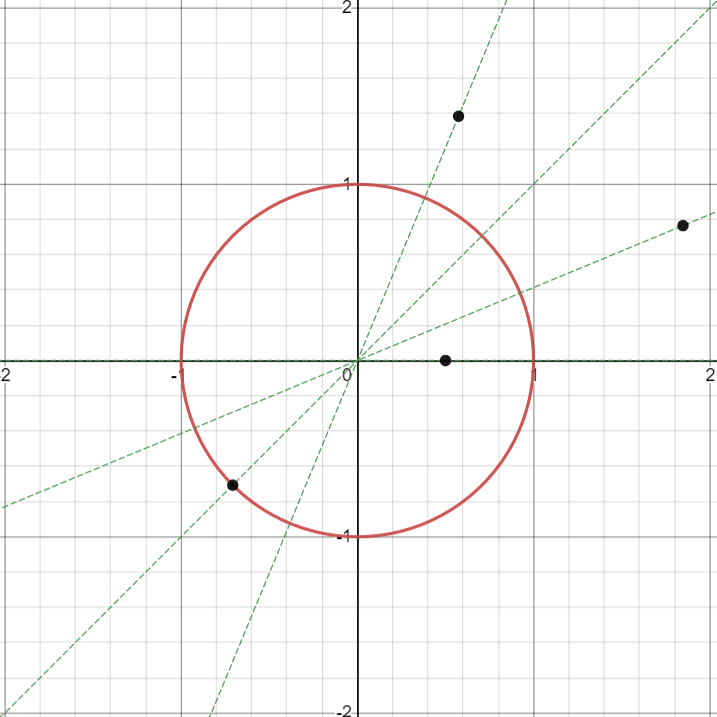
\includegraphics[width=6cm]{furier}
    \caption{Wizualizacja powstawania transformaty Fouriera dla $X=\left[0.5,\ 2,\ -1,\ 1.5,\ \dots\right]$, wykonana w aplikacji Desmos}
    \label{fig:fourier_vis}
\end{figure}
gdzie $i = \sqrt{-1}$. Jej idea opiera się na umieszczeniu punktów wokół początku układu współrzędnych tak, żeby miary kątowe między kolejnymi punktami były identyczne, a odległości od początku układu współrzędnych równe wartościom wektora $X$ (jak możemy zobaczyć na rysunku \ref{fig:fourier_vis}), a następnie obliczeniu średniej pozycji tych punktów. W celu przeprowadzenia testu musimy przyjąć następujące twierdzenia:
\begin{itemize}
    \item Zarówno $\sqrt{\frac{2}{t}} Im(Y_k)$ oraz $\sqrt{\frac{2}{t}} Re(Y_k)$ przy $t \to \infty$ mają rozkład normalny $\mathcal{N}\left(0, 1\right)$,
    \item Zarówno $\sqrt{\frac{2}{t}} Im(Y_k)$ oraz $\sqrt{\frac{2}{t}} Re(Y_k)$ przy $t \to \infty$ są od siebie niezależne,
\end{itemize}
gdzie $Re(z)$ zwraca część rzeczywistą liczby zespolonej, a $Im(x)$ oznacza wartość urojoną liczby. Dowód tych twierdzeń odnaleźć można w pracy \emph{Randomness evaluation with the discrete fourier transform test basedon exact analysis of the reference distribution} \cite{Fourier_test}. Mając te dwa rezultaty możemy w łatwy sposób wywnioskować, iż:
\begin{equation}
    \frac{2}{n}|Y_k|^2 \sim \chi^2_2 \textrm{(rozkład chi kwadrat z 2 stopniami swobody)}
\end{equation}
Znając dokładny rozkład dla $\frac{2}{n}|Y_k|^2$, przy $n \to \infty$ możemy się podjąć się wyznaczenia wartości krytycznej $\kappa$:
\begin{equation}
    \begin{split}
        P(|Y_k| \leq \kappa) &= 0.95\\
        \int_0^{\frac{2}{n}\kappa^2}\frac{1}{2}e^{-\frac{y}{2}}dy &= 0.95\\
        1 - e^{-\frac{\kappa}{n}} &= 0.95\\
        \kappa &= \sqrt{-n\ln{(0.05)}}
    \end{split}
\end{equation}
Ze względu na własność $|Y_k| = |\overline{Y_{N-k}}|$, wykonujemy testy jedynie dla $k \leq \frac{n}{2}$. Ponieważ ten test składa się z $\frac{n}{2}$ testów szansa, że wszystkie z nich przejdą pomyślnie test wynosi $0.95^{\frac{n}{2}}$, co szybko dąży do 0. Dlatego też przy ocenie rezultatu testu musimy pamiętać o tym, iż 5\% z nich powinno uzyskać wynik negatywny. Mamy więc do czynienia z rozkładem Bernuliego.
\begin{equation}
    Z \sim \mathcal{B}(\frac{n}{2}, 0.95)
\end{equation}
Jest to znany rozkład, którego parametry wynoszą:
\begin{equation}
    \begin{split}
        \mathbb{E}Z &= \frac{n}{2}0.95\\
        Var(Z) &= \frac{n}{2}(0.05)(0.95)
    \end{split}
\end{equation}
Możemy zatem korzystając z centralnego twierdzenia granicznego przybliżyć go rozkładem normalnym:
\begin{equation}
    \mathcal{N}\left(\frac{n}{2}0.95, \frac{n}{2}(0.05)(0.95)\right)
\end{equation}
\subsubsection{Wartość $p$}
Celem ustalenia wartości $p$ najpierw dokonamy szybkiej transformaty Fouriera na wektorze bitów zmapowanym funkcją $f(x) = 2x - 1$ (a więc zmieniającą 0 na -1), po czym wyliczamy wektor $r$:
\begin{equation}
    r_k =[\![|Y_k| < \sqrt{-n\ln{(0.05)}}]\!]
\end{equation}
gdzie $[\![$\emph{wyrażenie}$]\!]$ jest funkcją prawdy i przyjmuje 1 (jeśli zdanie jest prawdziwe) i 0 (w przeciwnym wypadku).
\begin{equation}
    P_{\textrm{value}} = 1 - \textrm{erf}\left(\frac{|\sum_{j=0}^{\frac{n}{2}r_k} - \mathbb{E}Z|}{\sqrt{2Var(Z)}} \right)
\end{equation}
Test uznajemy za zaliczony jeśli $P_{\textrm{value}} > 0.05$.
\subsection{Test nakładających się wzorców}
\subsubsection{Cel testu}
Celem testu jest sprawdzenie, czy wstępowanie danego wzorca $B = b_1b_2b_3\dots b_m$ w otrzymanym wektorze pokrywa się z teoretycznym rozkładem przy założeniu jego jednostajności oraz niezależności.
\subsubsection{Matematyczne uzasadnienie}
Obliczenie dokładnego prawdopodobieństwa dla poszczególnej liczby występowania wzorca $B$ w losowym wektorze $X=x_1x_2x_3\dots x_n$ jest bardzo trudnym zadaniem. Możemy poznać dokładne wartości dla wzorców długości 4 \cite{4bits_patterns}, jednak samo wyliczenie wszystkich prawdopodobieństw jest niełatwe ze względu na złożoność obliczeniową. Stąd też użyjemy oszacowania rozkładem normalnym. Żeby to zrobić, musimy najpierw wyznaczyć wartość oczekiwaną oraz wariancję. Aby je obliczyć potrzebujemy nowego wektora zmiennych losowych.
\begin{equation}
    \label{vect_pos}
    Y_k = [\![ x_{k-m+1}x_{k-m+2}\dots x_k = b_1b_2\dots b_m]\!]
\end{equation}
Wektor $Y$ z definicji \ref{vect_pos} informuje nas, czy na $k$-tej pozycji kończy się poszukiwany przez nas wzorzec. Z łatwością możemy obliczyć, że dla każdego $k \in \{m, \dots, n\} Y_k = \frac{1}{2^m}$. Oznaczmy zmienną losową liczbę występowania wzorca $B$ w losowym wektorze jako $Q$. Zatem:
\begin{equation}
    \label{patern_expected}
    \mathbb{E}Q = \mathbb{E}{\sum_{k=m}^n Y_k}=\sum_{k=m}^n \mathbb{E}Y_k = \sum_{k=m}^n \frac{1}{2^m} = \frac{n-m+1}{2^m}
\end{equation}
Wzór \ref{patern_expected} wynika z faktu, iż wartość oczekiwana sumy jest zawsze sumą wartości oczekiwanych, przez co nie musimy przejmować się problemem zależności wektora $Y$. Prawo wariancji sumy jest bardziej skomplikowane:
\begin{equation}
    \label{sum_of_var}
    Var(A+B) = Var(A) + Var(B) + cov(A, B)
\end{equation}
Jak widzimy na wzorze \ref{sum_of_var}, aby policzyć sumę wariancji konieczne jest ustalenie kowariancji zmiennych losowych. Kowariancję definiujemy wzorem \ref{eq:cov_def}.
\begin{equation}
    \label{eq:cov_def}
     cov(A, B) = \mathbb{E}[(A -\mathbb{E}A)(B - \mathbb{E}B)] = \mathbb{E}[AB] - \mathbb{E}A\mathbb{E}B
\end{equation}
Aby wyliczyć wartość wariancji dla $\sum_{k=m}^n Y_k$, zastosujemy proces iteracyjny. Najpierw wyliczymy $Var(Y_m + Y_{m+1})$, następnie $Var((Y_m + Y_{m+1}) + Y_{m+2})$, żeby na samym końcu poznać wartość $Var(\sum_{k=m}^{n-1} Y_k+ Y_{n})$. Musimy być zatem w stanie ustalić wartość wyrażenia \ref{eq:e_sum_x} dla każdego $t$.
\begin{equation}
    \label{eq:e_sum_x}
    \mathbb{E}\left[Y_t\sum_{k=m}^{t-1}Y_k\right] = \mathbb{E}\left[\sum_{k=m}^{t-1}Y_t Y_k\right] = 
    \sum_{k=m}^{t-1}\mathbb{E}\left[Y_t Y_k\right]
\end{equation}
Ponieważ $Y$ jest wektorem zer i jedynek oraz $0x = 0$ możemy wzór \ref{eq:e_sum_x} zapisać w formie wyrażenia \ref{eq:e_sum_x_simpl}, pomijając zbędne zera.
\begin{equation}
    \label{eq:e_sum_x_simpl}
    \sum_{k=m}^{t-1}\mathbb{E}\left[Y_t Y_k\right] =
    \sum_{k=m}^{t-1}\mathbb{E}\left[Y_k | Y_t = 1\right] P(Y_t = 1) = 
    \sum_{k=m}^{t-1}\mathbb{E}\left[Y_k | x_{k-m+1}\dots x_k = b_1\dots b_m \right]P(Y_t = 1)
\end{equation}
Widzimy zatem, iż musimy obliczyć oczekiwaną liczbę wzorców $B$ w wektorze długości $t-1$ znając ostanie $m-1$ pozycji tego wektora. Dla $Y_m, \dots, Y_{t-m}$ wartość oczekiwana się nie zmienia i wynosi $\frac{1}{2^m}$. Dla pozostałych $Y_{t-m+1}, \dots, Y_{t-1}$ natomiast koniecznym będzie wyliczenie wartości, które zależą one od samego wzorca $B$. Kończąc, przemnożymy otrzymaną wartość oczekiwaną przez prawdopodobieństwo, że $Y_t = 1$, a więc przez $\frac{1}{2^m}$.
\subsubsection{Wartość $p$}
Wzorzec $B$ jest nam dany. Pierwszym krokiem będzie wyliczenie jego wartości oczekiwanej $\mathbb{E}Q$, wariancji $Var(Q)$ oraz liczby wystąpień wzorca (do której ustalenia najlepiej zastosować algorytm Knutha-Morrisa-Pratta), oznaczonej $Q$. Podstawiając do wzoru, otrzymujemy:
\begin{equation}
    P_{\textrm{value}} = 1 - \textrm{erf}\left(\frac{|Q - \mathbb{E}Q|}{\sqrt{2Var(Q)}} \right)
\end{equation}
Test uznajemy za zaliczony jeśli $P_{\textrm{value}} > 0.05$.
\subsection{Test złożoności liniowej}
\subsubsection{Cel testu}
W tym teście skupimy się na sprawdzeniu jak dobrze złożoność liniowa $M$-bitowych bloków wektora losowego pokrywa się z oczekiwanymi rezultatami. Złożoność linową zdefiniujemy jako najkrótszy rejestr przesuwający z liniowym sprzężeniem zwrotnym (dalej \emph{LFSR}) który może wygenerować ten ciąg. W celu obliczenia złożoności liniowej bloku wykorzystamy algorytm Berlekampa–Masseya \cite{mass}.
\subsubsection{Matematyczne podstawy testu}
Wyznaczmy teoretyczny rozkład złożoności linowej $\Lambda$ przy założeniu jednostajności i niezależności. Obliczenia zostały oparte na pracy R. A. Rueppela \cite{expected_lfsr}. Dla każdego ciągu $n$-bitów $s^n$ możemy wyliczyć jego złożoność linową $\Lambda(s^n)$. Korzystając z pracy J. Masseya \cite{mass} wiemy, że zachodzi następująca zależność rekurencyjna:
\begin{equation}
\label{eq:req_lfsr}
    \Lambda(s^{n+1}) = \begin{cases} 
    \Lambda(s^n) & \textrm{jeśli najkrótszy LFSR dla $s^n$ produkuje odpowiedni bit}\\
    \Lambda(s^n) & \textrm{jeśli najkrótszy LFSR dla $s^n$ nie jest odpowiedni, ale $ \Lambda(s^n) \geq \frac{n}{2}$}\\
    n -\Lambda(s^n) & \textrm{jeśli najkrótszy LFSR dla $s^n$ nie jest odpowiedni i $ \Lambda(s^n) < \frac{n}{2}$}\\
    \end{cases}
\end{equation}
Oznaczmy teraz liczbę ciągów długości $n$ o złożoności liniowej $L$ jako $N_n(L)$. Ciąg $s^{n+1}$ składa się z ciągu $s^{n}$ z dodanym jednym bitem. Jeśli ten dodatkowy bit odpowiada już istniejącemu najkrótszemu \emph{LFSRowi}, jego złożoność się nie zmienia. Dla przypadku kiedy $\Lambda(s^{n+1}) = L' < \frac{n}{2}$, ponieważ złożoność liniowa nie może spaść po dodaniu bitu, do tej kategorii zaliczymy jednie ciągi $n$ bitów, którym dodano odpowiadający bit, zatem $N_{n+1}(L')= N_{n}(L')$. Ciągi, którym dodano nieodpowiadający bit zmienią swoją złożoność. Dlatego też w przypadku $L' > \frac{n+1}{2}$ liczba takich ciągów wyniesie $N_{n}(n-L')$ (są to te którym wzrosła złożoność) plus $2N_{n}(L')$ (ponieważ dla $ \Lambda(s^n) \geq \frac{n+1}{2}$ złożoność się nie zmienia). W przypadku $L' = \frac{n+1}{2}$ ciągi o długości $n$ z dodanym dowolnym bitem zachowają swoją złożoność, więc $N_{n+1}(L') = 2N_{n}(L')$.
\begin{equation}
\label{eq:num_of_lfsr}
    N_{n+1}(L) = \begin{cases} 
    2N_{n}(L)+N_{n}(n-L) & \textrm{jeśli } L > \frac{n+1}{2}\\
    2N_{n}(L) & \textrm{jeśli } L = \frac{n+1}{2}\\
    N_{n}(L)  & \textrm{jeśli } L < \frac{n+1}{2}\\
    \end{cases}
\end{equation}
Wzór \ref{eq:num_of_lfsr} możemy uprościć do formy \ref{eq:lfsr_simp}, której dowód znaleźć możemy w pracy R. A. Rueppela \cite{expected_lfsr}.
\begin{equation}
\label{eq:lfsr_simp}
    N_{n}(L) = \begin{cases} 
    1 & \textrm{jeśli } n \geq L > 0\\
    2^{\{2n-2L, 2L - 1\}} & \textrm{w przeciwnym przypadku}\\
    \end{cases}
\end{equation}
 Ze względu na dużą dysproporcję w ilości ciągów dla odpowiednich złożoności, zastosujemy grupowanie wyników w $T$-przedziałów o różnej długości dla $M$=1024 ($[0, 255]$, $\dots$, $[510, 511]$, $[512]$, $[513, 514]$, $\dots$, $[786, 1024]$). Zastosujemy zatem test $\chi^2$ Petersona:
\begin{equation}
    \chi^2 = N\sum_{k=0}^{T-1}{\frac{(\frac{O_k}{N}-p_k)^2}{p_k}}
\end{equation}
gdzie:
\begin{description}
    \item[$N$] - liczba $M$-bitowych rozłącznych przedziałów,
    \item[$T$] - liczba kategorii,
    \item[$O_k$] - liczba przedziałów zaliczonych do $k$-tej kategorii,
    \item[$p_k$] - prawdopodobieństwo przynależności do $k$-tej kategorii.
\end{description}
\subsubsection{Wartość $p$}
Test rozpoczynamy od wyznaczania prawdopodobieństwa $p$ dla każdej z kategorii. Następnie dzielimy wektor $X$ na $M$-bitowe bloki. Korzystając z algorytmu Berlekampa–Masseya wyliczamy ich złożoności i dodajemy do odpowiedniej kategorii $O$. Następnie obliczamy wartość $p$:
\begin{equation}
    P_{\textrm{value}} =  1-\Psi_{(T-1)}\left(N\sum_{k=0}^{T-1}{\frac{(\frac{O_k}{N}-p_k)^2}{p_k}}\right)
\end{equation}
Za pozytywy wynik uznajemy $P_{\textrm{value}} > 0.05$.
\subsection{Test ostatniego przecięcia}
\subsubsection{Cel testu}
Test skupia się na sprawdzeniu, kiedy po raz ostatni losowa ścieżka wygenerowana na podstawie wektora losowego $X$ długości $n$ osiągnie wartość zero (innymi słowy kiedy po raz ostatni wyrówna się ilość zer i jedynek w wektorze $X$), a następnie porównaniu tej wartości do teoretycznego rozkładu. 
\subsubsection{Matematyczne podstawy}
Pierwszym krokiem w wyznaczeniu ostatniego punku osiągnięcia 0 będzie zdefiniowanie wektora $Y$, który określa naszą pozycję w kroku $t$:
\begin{equation}
    Y_t = \sum_{k=0}^{t-1}(2X_k-1)
\end{equation}
Naszym celem jest wyznaczenie największego $t$ takiego, że $Y_t = 0$. Dla znanego wektora $X$ obliczenie tej wartości jest prostym zadaniem o złożoności obliczeniowej $O(n)$. Aby przeprowadzić test musimy jednak poznać również teoretyczny rozkład ostatniego przecięcia dla wektorów długości o $n$. Posłużymy się zatem centralnym twierdzeniem granicznym, które pozwoli nam oszacować ten ruch jednowymiarowym ruchem Browna (ściślej: procesem Weinera). Dla takich ruchów możemy zastosować drugie prawo \emph{arcus sinusa}, które brzmi:
\begin{equation}
    \label{eq:arcsin_law}
    P(L \leq x) = \frac{2}{\pi}\arcsin(\sqrt{x})
\end{equation}
gdzie $L$ oznacza ostatni punkt w którym ruch Browna przyjmuje wartość 0. Dowód twierdzenia \ref{eq:arcsin_law} możemy znaleźć w pracy \emph{Arcsine laws and its simulation and application} \cite{arcsin_laws}. Rozkład ten jest dojść płaski, a wartość oczekiwana nie pokrywa się z modą. W związku z tym dla $x \in [0, 1]$ podzielimy wektor $X$ na $N$ 2047-bitowych rozłącznych wektorów. Dodatkowo pogrupujemy wyniki na 16 kategorii, po czym zastosujemy test $\chi^2$ Petersona.
\begin{equation}
    \chi^2 = N\sum_{k=0}^{15}{\frac{(\frac{O_k}{N}-p_k)^2}{p_k}}
\end{equation}
gdzie:
\begin{description}
    \item[$N$] - liczba 2047-bitowych rozłącznych przedziałów, a więc $\lfloor \frac{n}{2047} \rfloor$,
    \item[$O_k$] - liczba przedziałów zaliczonych do $k$-tej kategorii, 
    \item[$p_k$] - prawdopodobieństwo przynależności do $k$-tej kategorii.
\end{description}
\subsubsection{Wartość $p$}
Rozpoczynamy obliczając prawdopodobieństwo dla każdej z kategorii:
\begin{equation}
    p_k = \frac{2}{\pi}\left(\arcsin\left(\sqrt{\frac{128(k+1)}{2048}}\right) - \arcsin\left(\sqrt{\frac{128k}{2048}}\right)\right)
\end{equation}
W kolejnym kroku dzielimy wektor na 2047-bitowe przedziały zliczając, ile wektorów należy do każdej kategorii. Następnie obliczamy wartość $p$:
\begin{equation}
    P_{\textrm{value}} =  1 - \Psi_{15}\left(N\sum_{k=0}^{15}{\frac{(\frac{O_k}{N}-p_k)^2}{p_k}}\right)
\end{equation}
Za pozytywy wynik uznajemy $P_{\textrm{value}} > 0.05$.
\subsection{Test największej sumy}
\subsubsection{Cel testu}
Test skupi się na wyznaczeniu maksymalnej wartości losowej ścieżki wygenerowanej w oparciu o $n$-bitowy wektor losowy $X$, po czym otrzymany wynik zostanie porównana do teoretycznego rozkładu tej zmiennej.
\subsubsection{Matematyczne podstawy}
Na początku przedstawimy kilka użytecznych definicji których użyjemy w dalszym rozumowaniu. Całość jest inspirowana notatkami z wykładu dostępnego pod adresem \cite{Max_Brown}.
\begin{equation}
    \begin{split}
        W_t &= \sum_{k=1}^{t}(2X_k - 1)\\
        T_a &= \min\{t \leq 0: W_t = a\} \\
        M_t &= \max_{0\leq k \leq t}W_k
    \end{split}
\end{equation}
Ze względu na jednostajność rozkładu oraz niezależność, możemy dodatkowo powiedzieć, że: 
\begin{equation}
 \label{eq:dual_brown}
    P(W_t > a | T_a < t) =  P(W_t < a | T_a < t) = \frac{1 - P(W_t = a)}{2}
\end{equation}
Równanie \ref{eq:dual_brown} mówi, że jeśli wiemy, że w jakimś punkcie $T_a$ osiągnęliśmy wartość $a$ to szansa, że jesteśmy poniżej tej wartości jest identyczna jak ta, że jesteśmy powyżej jej. Dodatkowo, z definicji możemy wyczytać, że:
\begin{equation}
\label{eq:m_eq_t}
    (\forall t \in \mathbb{N})(\forall \in \mathbb{N})M_t \geq a \Longleftrightarrow T_a \leq t
\end{equation}
czyli, że jeśli maksimum do punktu $t$ jest większe od $a$ to w którymś punkcie przed $t$ nasz ruch musiał przyjąć wartość $a$.
\begin{equation}
\label{eq:brown_max}
    \begin{gathered}
    P(T_a \leq t) =\\
    =P(T_a \leq t \land W_t>a)+P(T_a \leq t \land W_t<a)+P(T_a \leq t \land W_t=a) = \\
    =2P(T_a \leq t \land W_t>a) + P(T_a \leq t \land W_t=a) =\\
    =2P(M_t \geq a \land W_t>a) + P(W_t=a) =\\ 
    =2P(W_t>a) + P(W_t=a)
    \end{gathered}
\end{equation}
W równaniu \ref{eq:brown_max} sprowadziliśmy problem znalezienia rozkładu największej wartości w naszej ścieżce do znalezienia rozkładu wartości w punkcie $t$. Ma on znany rozkład dwumianowy Bernoulliego. My natomiast przybliżmy go rozkładem normalnym korzystając z centralnego twierdzenia granicznego. Możemy zatem ponownie skorzystać z \ref{eq:bin_norm}.
\begin{equation}
    P(M_t \geq a) = P\left(\frac{M_t}{\sqrt{t}} \geq \frac{a}{\sqrt{t}}\right) = 2P\left(\frac{W_t}{\sqrt{t}} \geq \frac{a}{\sqrt{t}}\right) = 2\left(1 - \Phi\left(\frac{a}{\sqrt{t}}\right)\right)
\end{equation}
\subsubsection{Wartość $p$}
Pierwszym krokiem jest znalezienie największej wartości w losowej ścieżce ($M_n$). Podstawiając ją do wzoru otrzymamy wartość $p$:
\begin{equation}
    P_{\textrm{value}} = 1 - \textrm{erf}\left(\frac{M_n}{\sqrt{2n}}\right)
\end{equation}
Jeśli $P_{\textrm{value}} > 0.05$, to uznajemy test za zaliczony.
\subsection{Test rang macierzy}
\subsubsection{Cel testu}
Celem testu jest sprawdzenie złożoności linowej wektora losowego. W tym celu stworzymy losowe macierze binarne wymiaru $m \times m$, a następnie wyznaczymy ich rangi. Porównamy otrzymane wynik z ich teoretycznym rozkładem dla prawdziwie losowej macierzy.
\subsubsection{Matematyczne podstawy}
Aby przeprowadzić ten test, musimy najpierw wyznaczyć prawdopodobieństwo otrzymania losowej macierzy o wymiarach $m \times m$ z rangą $r$. Zadanie to zaczniemy od wyznaczenia prawdopodobieństwa, iż wektor losowy długości $m$ będzie liniowo zależny od zbioru wektorów o randze $(m - k)$. Wiemy, że dla przestrzeni liniowej o $k$ wymiarach wyznaczonej przez wektory $\mathcal{V} = (v_1, v_2, \dots, v_t)$ możemy znaleźć bazę $\mathcal{U} = (u_1, u_2, \dots, u_k)$, która tworzy identyczną przestrzeń, a wektory są parami rozłączne, co oznacza że jeśli jeden wektor na $t$-tej pozycji posiada jedynkę, to wszystkie pozostałe na $t$-tej pozycji mają zero, formalny zapis w następującej formule:
\begin{equation}
\label{eq:pair_disjoint}
    \begin{gathered}
        u_i = (u_i^1, u_i^2, \dots, u_i^m)\\
        (\forall i, j) u_i^j = 1 \rightarrow (\neg \exists t \not = i) u_i^t = 1
    \end{gathered}
\end{equation}
Aby nowy wektor $q$ był liniowo zależny od bazy $\mathcal{U}$ muszą zachodzić własności \ref{eq:line_dependency_1} oraz \ref{eq:line_dependency_2}:
\begin{equation}
    \label{eq:line_dependency_1}
    (\forall i) q \mathbin{\&} u_i = 0 \lor q \mathbin{\&} u_i = u_i\\
\end{equation}
\begin{equation}
    \label{eq:line_dependency_2}
    (\forall i) q \mathbin{\&} \overline{\left(\sum_{i=1}^{k} u_i \right)} \not= 0
\end{equation}
gdzie $\mathbin{\&}$ oznacza iloczyn bitowy dwóch wektorów, operację sumy dwóch wektorów zdefiniujemy jako ich sumę bitową, a $\overline{a}$ oznacza negację bitową wektora $a$. 
Gdyby nie zachodziła własność \ref{eq:line_dependency_1} (a więc istnieje wektor $u_i$, który pokrywa się jedynie w części z wektorem $q$), to niemożliwym jest stworzenie za pomocą operacji sumy rozłącznej z wektorów bazy $\mathcal{U}$ wektora $q$. Gdybyśmy dodali do sumy rozłącznej wektor $u_i$ nastąpiłoby dodanie bitów, które nie należą do $q$ sumy, natomiast jego nie dodanie spowodowałoby, że część bitów, które powinny być jedynką pozostaną zerem. 
Jeśli natomiast nie zachodziłoby \ref{eq:line_dependency_2} koniecznym byłoby ustawienie bitu, który nie jest jedynką w żadnym wektorze z bazy $\mathcal{U}$, co jest niemożliwe.
Z tych własności możemy wyciągnąć wniosek, iż dla bazy $\mathcal{U}$, istnieje $2^k$ wektorów zależnych, a prawdopodobieństwo wylosowania takiego wektora wynosi $\frac{2^{k}}{2^{n}}$ 
Pozostaje nam zatem wyliczyć prawdopodobieństwo uzyskania macierzy wymiaru $m \times m$ o randze $(m - k)$. Wiemy, iż została zbudowana z $k$ liniowo zależnych oraz $(m-k)$ liniowo niezależnych rzędów. Prawdopodobieństwo otrzymania liniowo niezależnego wektora zależy jedynie od rangi poprzednich wierszy. Niezależnie od ich pozycji stanowią one człon $\prod_{i=0}^{m-k-1}(1-2^{-(m-i)})$. Pozostaje nam jeszcze wyliczenie drugiego członu, a więc prawdopodobieństwo wylosowania $k$ liniowo zależnych wierszy. Niestety, ich pozycja ma wpływ na prawdopodobieństwo, przez co zmuszeni jesteśmy zsumować wszystkie kombinacje. Ostatecznie wzór \ref{eq:prob_of_matrix} wyznacza prawdopodobieństwo uzyskania losowej macierzy $m\times m$ o randze $(m-k)$. Dokładny dowód można znaleźć w książce \emph{Random graphs} \cite{kolchin_1998}. 
\begin{equation}
    \label{eq:prob_of_matrix}
    P_m(k) = 2^{-k^2}\left(\prod_{i=0}^{m-k-1}(1-2^{-(m-i)})\right)\left(\sum_{0\leq i_1\leq\dots i_k\leq m-k}2^{-(i_1+i_2+\dots + i_k)}\right)
\end{equation}
Formuła \ref{eq:prob_of_matrix} jest niestety wymagająca obliczeniowo, w związku z tym wyniki podzielimy na 10 kategorii: $k=0$, $k=1$, $\dots$, $k=8$, $k > 8$, a następnie wykonamy test $\chi^2$ Petersona.
\begin{equation}
    \chi^2 = N\sum_{k=0}^{9}{\frac{(\frac{O_k}{N}-p_k)^2}{p_k}}
\end{equation}
gdzie:
\begin{description}
    \item[$N$] - liczba macierzy $m\times m$,
    \item[$O_k$] - liczba przedziałów zaliczonych do $k$-tej kategorii, 
    \item[$p_k$] - prawdopodobieństwo przynależności do $k$-tej kategorii wyliczone na podstawie wzoru \ref{eq:prob_of_matrix}.
\end{description}
\subsubsection{Wartość $p$}
Pierwszym krokiem jest wyliczenie teoretycznego prawdopodobieństwa dla każdej z dziesięciu kategorii, ustalenie rangi każdej macierzy oraz dodanie jej do odpowiedniej kategorii $O_i$. Następnie wyliczamy wartość $\chi^2$, oraz wartość $p$:
\begin{equation}
    P_{\textrm{value}} =  1 - \Psi_{9}\left(N\sum_{k=0}^{9}{\frac{(\frac{O_k}{N}-p_k)^2}{p_k}}\right)
\end{equation}
Przy wartości $P_{\textrm{value}} > 0.05$ uznajemy test za zaliczony.

\section{Wyniki testów}
Po zapoznaniu się z metodami testowania możemy przeanalizować uzyskane wyniki.
\subsection{Wyniki naszych testów}
Na podstawie przedstawionych powyżej testów stworzyliśmy program sprawdzający losowość w języku Python. Do testów wykorzystaliśmy 12 megabajtowe wektory losowych bitów wygenerowane przez odpowiednie generatory. Test jedynek w bloku oraz test najdłuższego ciągu dla bloków 1024 bitów zostały zmodyfikowane poprzez połączenie mało prawdopodobnych kategorii w jedną większą w celu zminimalizowania błędów numerycznych. Pozostałe testy zostały zaimplementowane bez żadnych zmian.
\begin{table}[!ht]
    \centering
    \begin{tabular}{|l|c|c|c|c|}
    \hline
        \textbf{Nazwa testu} & \textbf{LCM} & \textbf{Tarus} & \textbf{CRNG} & \textbf{Nasz generator} \\ \hline
        Test częstotliwości & 0.12882 & 0.68573 & 0.51296 & 0.11257 \\ \hline
        Test jedynek w bloku (128) & \cellcolor{lred} 0.00000 & 1.00000 & 1.00000 & 1.00000 \\ \hline
        Test jedynek w bloku (1024) & \cellcolor{lred}0.00000 & 0.76419 & 0.86979 & 0.68492 \\ \hline
        Test nieprzerwanych ciągów & 0.65722 & 0.78955 & \cellcolor{lred}0.04002 & 0.58470 \\ \hline
        Test najdłuższego ciągu (64) & \cellcolor{lred}0.00000 & 0.99966 & 0.99996 & 1.00000 \\ \hline
        Test najdłuższego ciągu (1024) & \cellcolor{lred}0.00000 & 0.99826 & 0.69517 & 0.99922 \\ \hline
        Test nieokresowości & \cellcolor{lred}0.00000 & 0.86880 & 0.75849 & 0.27542 \\ \hline
        Test nakładających się wzorców & 0.48773& 0.97426& 0.27960& 0.82126 \\ \hline
        Test złożoności liniowej & 0.99864 & 0.925021 & 0.99146 & 0.99740 \\ \hline
        Test ostatniego przecięcia & \cellcolor{lred}0.00000 & 0.89303 & 0.98706 & 0.83454 \\ \hline
        Test największej sumy & 0.06399 & 0.52433 & 0.71036 & 0.47557 \\ \hline
        Test rang macierzy (32x32) & 0.84882 & 0.92983 & 0.96152 & 0.94216 \\ \hline
        Test rang macierzy (16x16) & 0.85061 & \cellcolor{lred}0.00308 & 0.99792 & 0.97909 \\ \hline
    \end{tabular}
    \caption{\label{tab:my_res}Wyniki naszych testów dla różnych generatorów wuwzględniające wartości $p$ dla poszczególnych testów. Z wyróżnieniem wyniki gdzie wartość $p$ jest mniejsza od poziomu istotności $\alpha = 0.05$}
\end{table}
Jak widzimy w tablicy \ref{tab:my_res} najgorzej poradził sobie generator \emph{LCM}, co jest spodziewane z uwagi na jego prymitywną konstrukcję. Wyniki generatora \emph{Tarus} oraz \emph{CRNG} są bardzo zbliżone, co może dziwić z względu na to, iż generator \emph{CRNG} powinien znacząco lepszej klasy. Najlepiej w testach wypadł nasz generator. Z uwagi, iż testy opierają się na testach statystach nie można wyciągnąć jednak jednostajnych wniosków na temat jego wyższości nad \emph{CRNG}.
\subsection{Wyniki testów narzędziem \textit{Diehard}}
Dodatkowo, wykorzystując narzędzie \emph{Diehard} \cite{Diehard}, przeprowadziliśmy kolejne testy. Dla każdego z nich zwracającego więcej niż jedną wartość $p$, w tablicy \ref{tab:diehard} została zaprezentowana ostatnia z nich.
\begin{table}[!ht]
    \centering
    \begin{tabular}{|l|c|c|c|c|}
    \hline
        \textbf{Nazwa testu} & \textbf{LCM} & \textbf{Tarus} & \textbf{CRNG} & \textbf{Nasz generator} \\ \hline
        Birthday Spacings & \cellcolor{lred}1.00000 & 0.50792 & 0.71394 & 0.03742 \\ \hline
        Overlapping Permutations & 0.82591 & 0.02708 & \cellcolor{lred}0.00131 & 0.54635 \\ \hline
        Ranks of 32x32 matrices & 0.54445 & 0.75272 & 0.65900 & 0.53647 \\ \hline
        Ranks of 6x8 Matrices & \cellcolor{lred}1.00000 & 0.42814 & 0.59030 & 0.32594 \\ \hline
        Monkey Tests on 20-bit Words & \cellcolor{lred}0.00000 & 0.20653 & 0.66948 & 0.89925 \\ \hline
        Monkey Tests DNA & 0.34920 & 0.34380 & 0.86220 & 0.34810 \\ \hline
        Count the 1`s in a Stream of Bytes & \cellcolor{lred}1.00000 & 0.32245 & \cellcolor{lred}0.98657 & 0.48885 \\ \hline
        Count the 1`s in Specific Bytes & 0.74763 & 0.51252 & 0.59320 & 0.52139 \\ \hline
        Parking Lot Test & 0.53309 & \cellcolor{lred}0.02187 & 0.71684 & 0.10980 \\ \hline
        Minimum Distance Test & 0.62647 & \cellcolor{lred}0.00003 & 0.58250 & 0.90770 \\ \hline
        Random Spheres Test & 0.08858 & 0.94746 & 0.43352 & 0.77891 \\ \hline
        The Sqeeze Test & 0.10927 & 0.07114 & 0.35482 & 0.81188 \\ \hline
        Overlapping Sums Test & 0.89813 & 0.15546 & 0.86684 & 0.15546 \\ \hline
        Runs Test & 0.34953 & 0.35924 & 0.55256 & 0.91654 \\ \hline
        The Craps Test & 0.56509 & 0.69635 & 0.08896 & 0.65335 \\ \hline
    \end{tabular}
    \caption{\label{tab:diehard} Wyniki testów narzędziem \emph{Diehard} \cite{Diehard} dla różnych generatorów z uwzględnieniem wartości $p$ dla poszczególnych testów i wyróżnieniem wyników, gdzie wartość p znajduje się poza przedziałem ufności $0.025 < P_\textrm{value} < 0.975$ dla tego narzędzia}
\end{table}
Podobnie jak w przypadku poprzednich testów, tu również nasz generator wypadł najlepiej w porówaniu do wszystkich innych generatorów. Jest on wyraźnie lepszy od rozwiązania \emph{LCM}, jak również wydaje się być lepszy od dwuch pozostałych generatorów.
\subsection{Wyniki testów narzędziem \textit{NIST test suite}}
\begin{table}[!ht]
    \centering
    \begin{tabular}{|l|c|c|c|c|}
    \hline
        \textbf{Nazwa testu} & \textbf{LCM} & \textbf{Tarus} & \textbf{CRNG} & \textbf{Nasz generator} \\ \hline
        Frequency & 0.12233 & 0.91141 & 0.35049 & 0.12233 \\ \hline
        Block Frequency & \cellcolor{lred}0.00000 & 0.53415 & 0.53415 & 0.53415 \\ \hline
        Cumulative Sums & 0.53415 & 0.73992 & 0.35049 & 0.35049 \\ \hline
        Runs & 0.53415 & \cellcolor{lred}0.03517 & 0.35049 & \cellcolor{lred}0.03517 \\ \hline
        Longest Run & 0.21331 & 0.53415 & 0.12233 & 0.53415 \\ \hline
        Rank & 0.73992 & 0.53415 & 0.12233 & 0.53415 \\ \hline
        FFT & \cellcolor{lred}0.00000 & \cellcolor{lred}0.00888 & 0.53415 & 0.35049 \\ \hline
        Non Overlapping Template & \cellcolor{lred}0.03517 & 0.91141 & 0.21331 & 0.35049 \\ \hline
        Overlapping Template & \cellcolor{lred}0.00000 & 0.53415 & 0.06688 & 0.53415 \\ \hline
        Universal & \cellcolor{lred}0.00000 & 0.73992 & 0.73992 & 0.73992 \\ \hline
        Approximate Entropy & \cellcolor{lred}0.00000 & 0.21331 & 0.35049 & 0.73992 \\ \hline
        Serial & \cellcolor{lred}0.00000 & 0.91141 & 0.12233 & \cellcolor{lred}0.00430 \\ \hline
        Linear Complexity & 0.73992 & 0.35049 & 0.06688 & 0.21331 \\ \hline
    \end{tabular}
    \caption{\label{tab:nist}  Wyniki testów narzędziem \emph{NIST test suite}
 \cite{NISTTests} dla różnych generatorów z uwzględnieniem wartości $p$ dla poszczególnych testów i wyróżnieniem wyników, gdzie wartość p jest mniejsza od poziomu istotności $\alpha = 0.05$}
\end{table}
Z względu na przejrzysty interfejs narzędzia \emph{NIST test suite} \cite{NISTTests} przeprowadziliśmy dodatkowe testy z jego wykorzystaniem. Użyliśmy identycznych danych jak w dwóch poprzednich testach, podzielonych na 10 strumieni o długości 10000000 bitów każdy.  Dla spójności zastosowaliśmy poziom istotności $\alpha = 0.05$ (taki jak dla poprzednich testów), pomimo zalecanego $\alpha = 0.01$. W przypadku testów, które narzędzie wykonuje kilkukrotnie w celu poprawienia czytelności w tablicy \ref{tab:nist} zaprezentowano jedynie ostanie wyniki. Możemy w niej zobaczyć, że nasz generator wypada gorzej od generatora \emph{CRNG}. Szczególnie niepokoić może wynik testu \emph{Serial} dla którego wartość p wynosi 0.00430. Oznacza to, iż w jedynie 0.43\% przypadków poprawny generator wygeneruje tak skrajne wyniki. Tak jak w poprzednich testach najgorzej wypada \emph{LCM}. Generator \emph{Tarus} radzi sobie lepiej, jednak również nie przeszedł części testów. \emph{CRNG}, w przeciwieństwie do poprzednich narzędzi, przeszedł wszystkie testy bezbłędnie, jednak w wielu testach wartość $p$ znajdowała się na granicy przedziału ufności.